\documentclass[11pt]{article}
\usepackage{graphicx}
\usepackage{amssymb}
\usepackage{color}

\textwidth = 6.5 in
\textheight = 9 in
\oddsidemargin = 0.0 in
\evensidemargin = 0.0 in
\topmargin = 0.0 in
\headheight = 0.0 in
\headsep = 0.0 in
\parskip = 0.2in
\parindent = 0.0in


\begin{document}
{\large {\bf CMPT 202 - Searching}} 



%\begin{enumerate}

1. Why might we need to search for an item in an array/list?
\vspace*{0.5in}

 2. Consider the following array. Write the psuedocode for an algorithm for a {\it sequential search} that returns true if a given value occurs in the list, and false otherwise. \\

\begin{tabular}{|c|c|c|c|c|c|c|c|c|c|c|c|} \hline
115 & 67 & 0 & -200 & 54 & 99 & 12 & 42 & -42 & 15 & 60\\ \hline 
0 & 1 & 2 & 3 & 4 & 5 & 6 & 7 & 8 & 9 & 10 \\ \hline
\end{tabular} \\

{\tt boolean search(int[] array, int value) \{ } \\

\vspace*{1.0in}

\} 

3. Complete the following table using the sequential search with $N$ elements: 


\begin{tabular}{|c|c|} \hline
&   Number of Comparisons  \\ \hline 
Best case &  \\ \hline
Worst case &  \\ \hline
Average case &  \\ \hline
\end{tabular} \\

4. What is the Big-Oh notation of the sequential search?

\noindent
We can use a different algorithm if our data is in sorted order:

\begin{tabular}{|c|c|c|c|c|c|c|c|c|c|c|} \hline
-200 & -42 & 0 & 12 & 15 & 42 & 54 & 60 & 67 & 99 & 115 \\ \hline 
0 & 1 & 2 & 3 & 4 & 5 & 6 & 7 & 8 & 9 & 10 \\ \hline
\end{tabular} \\


5. What is the index and value at the midpoint of the list?

\vspace*{.25in}
 6. Suppose we are searching for 12, and we begin searching at the midpoint of the list. What can an algorithm take advantage of if the list is sorted?
%\vspace*{0.5in}


\newpage
\noindent
This is known as a {\it binary search}, and the general recursive algorithm is as follows:

{\tt // search for desiredItem in elements}  \\ 
{\tt binarySearch(elements, desiredItem) \{ } \\
\hspace*{.25in}{\tt // calculate midpoint} \\ \\
\hspace*{.25in}{\tt if (desiredItem == element at midpoint)} \\
\hspace*{.5in}{\tt we found it!!} \\
\hspace*{.25in}{\tt else  if (desiredItem < element at midpoint)} \\
\hspace*{.5in}{\tt search left side of elements} \\
\hspace*{.25in}{\tt else} \\
\hspace*{.5in}{\tt search right side of elements}  \\
\} \\

%\item Trace this algorithm searching for 12 in the above list.

%\noindent
%A more detailed sketch of the algorithm:

%{\tt // search for desiredItem in elements}  \\ 
%{\tt binarySearch(elements, desiredItem) \{ } \\
%\hspace*{.25in}{\tt midpoint = midway between 0 and (n-1)} \\ \\
%\hspace*{.25in}{\tt if (desiredItem == elements[midpoint])} \\
%\hspace*{.5in}{\tt return true} \\
%\hspace*{.25in}{\tt else  if (desiredItem < elements[midpoint])} \\
%\hspace*{.5in}{\tt return the result of searching  elements[0] through elements[midpoint-1]} \\
%\hspace*{.25in}{\tt else} \\
%\hspace*{.5in}{\tt return the result of searching  elements[midpoint+1] through elements[n-1]}  \\
%\} \\

 7. After proceeding through the worksheet, complete the following table using the binary search with the following size of $N$: 

\begin{tabular}{|c|c|c|c|c|c|} \hline
&   $N = 4$ & $N = 32$ & $N = 64$ & $N = 256$ & $N = 1024$   \\ \hline 
Max number of comparisons & & & & &   \\ \hline
\end{tabular} \\

8. What is the Big-Oh notation of the binary search?

Consider the following binary tree
\begin{figure}[h]
\centerline {
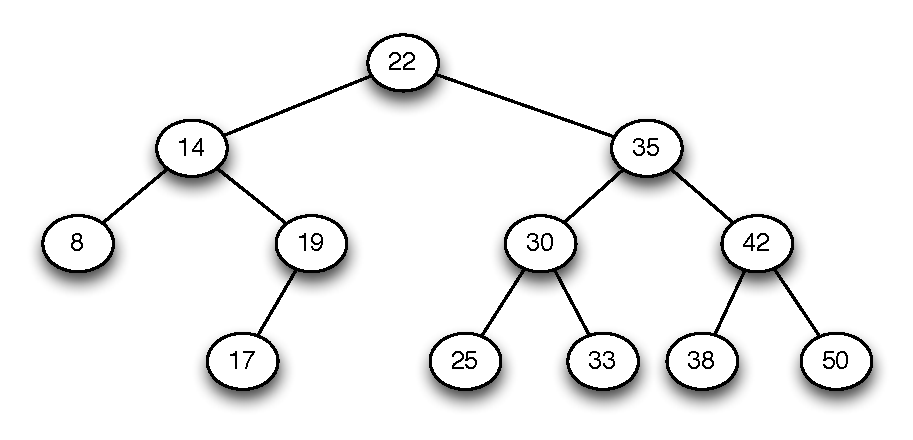
\includegraphics[width=5in]{TreeExerciseGraph.pdf}
}
\end{figure}

9. Explain how  binary search can be performed on a binary search tree. 
%\vspace*{0.5in}

 10. What is the height of a complete binary search tree with $N$ nodes?

 11. Explain how the shape of a binary search tree can influence its Big-oh performance.

%\end{enumerate}

 \end{document}
